\chapter{Peano coding patterns}

\section{Dynamic coarsening of the grid}

The operation \texttt{coarse} on a vertex may only be invoked on a refined
vertex.
Once it is called, all children recursively are removed.
Most naive codes realising dynamic adaptivity thus set the specification flag
\texttt{WholeTree} in some mapping where they check for erase candidates.
Though such an approach works fine, it often reduces the concurrency and speed
dramatically---notably if the actual algorithm works only on the finest grid
level. 
Also, it often is very dangerous to remove more than one grid level in one rush.


It is thus convenient to add checks which ensure that coarsening removes only
the finest grid.
Yet, your adaptivity criterion's mapping might specify that it acts
on the fine grid only but nevertheless might be invoked on the whole tree:
the fine grid specification is an optimisation hint to Peano. 
It is not a formal definition.
If you merge your refinement's mapping with another mapping or you run it 
on a very adaptive mesh, Peano might have to decide that it invokes the routines
on all grid levels.
It is thus convenient to specify that a refinement criterion is to be ran on the
finest grid only and, on top of this, check whether it applies to the finest
grid. 
In the example below, a refinement criterion would return \texttt{Coarsen} if
and only if it is invoked on an unrefined vertex.
We explain this idea further below.


To bring both things together---fine grid work and erases---one can, in this
context, exploit the fact that also fine grid events have access to the next
coarser level.
It is thus convenient to do some fine grid checks and then call erase on coarser
levels.
This way, you remove at most one level per grid sweep. 

\begin{code}
if (fineGridVertex.getRefinementControl()==Vertex::Records::Unrefined) {
 switch (getRefinementCommand(
   fineGridX,...,coarseGridVerticesEnumerator.getLevel()+1,
   fineGridVertex.getRefinementControl()==Vertex::Records::Unrefined
 )) { 
  case RefinementCommand::Coarsen:
   {
    // should hold if and only if vertex is unrefined
    dfor2(k)
     if (
      coarseGridVertices[coarseGridVerticesEnumerator(k)].getRefinementControl()
        ==Vertex::Records::Refined
      &&
      coarseGridVertices[coarseGridVerticesEnumerator(k)].isInside()
      &&
      getRefinementCommand(
       coarseGridVerticesEnumerator.getVertexPosition(k),...
      ) == RefinementCommand::Coarse
     ) {
      coarseGridVertices[coarseGridVerticesEnumerator(k)].erase();
     }
    enddforx
   }
   break;
   case RefinementCommand::Refine:
    fineGridVertex.refine();
    break;
 }
}
\end{code}

\noindent
The above snippet assumes that there is a function \texttt{getRefinementCommand} that identifies
  regions that are to be coarsened via a enumeration
  \begin{code}
  enum class RefinementCommand {
    Nop, Refine, Coarsen
  };
  \end{code}
\noindent

At a first glance, it seems that the routine is overspecified as it checks for
\linebreak
\texttt{getRefinementCommand==RefinementCommand::Coarsen} twice. However, this
is on purpose. 
We check whether a fine grid vertex is ``too fine'' with the first check.
If this holds, we check whether a coarsening criterion also would hold for the
next coarser vertices.
We also validate that a coarse grid vertex is refined.
The latter check ensures that we do not call coarse on unrefined vertices in
adaptive grid regions.

The cascade of coarsen checks has proven of value in many applications: If we
did coarsen all coarse grid vertices of one vertex that is ``too fine'', many
refinement criteria induce oscillations.
The coarsening is very aggressive and then most criteria find that too many
vertices have been removed and re-add them.
This can be very cumbersome.
Our nested checks ensure that no such oscillation an happen (for all refinement
criteria we have checked).



\section{Global statistics}

Global statistics, such as total number of cells, are typically held within the
state. So I do model them as attribute in \texttt{State.def} and mark them both
as \texttt{persistent} and as \texttt{parallelise}. The latter flag ensures that
the attributes are exchanged via MPI, too. Once the fields are added to the
\texttt{def}-file and we have regenerated the records, a typical analysis of
such global data then reads as follows:

\begin{enumerate}
  \item I add several \texttt{getXXX} routines to the \texttt{myproject::State}
  class that allow the reader to analyse the global attributes. 
  \item I add a routine \texttt{clearStatistics()} to \texttt{myproject::State}.
  It sets all the analysed data to zero (or different default values).
  \item In the runner, I invoke \texttt{clearStatistics()} on the repository's
  state just before I trigger \texttt{iterate}.
  \item The real semantics of the analysis is realised through a routine
  \texttt{mergeStatistics(const State\& otherState)} in the \texttt{State}. It
  is invoked on a state object and receives another state object. The data from the
  other state object is merged into the current state. This merge typically is a
  summation, maximum, minimum, \ldots
  \item I next program a serial version of the mapping conducting the actual
  analysis:
  \begin{enumerate}
    \item The mapping is given a new attribute \texttt{State \_localState}. The
    idea is that each mapping works with its local version of the state. This
    helps us later to avoid data races.
    \item The mapping's \texttt{beginIteration} invokes
    \texttt{clearStatistics} on \texttt{\_localState}. This clears the local
    data at the begin of the traversal.
    \item I next add routines in the mappings to count the statistics. This
    might for example be a statement in \texttt{enterCell} that increases cell
    counters. These statements all alter \texttt{\_localState}. 
    \item So far, the mapping only works on its local copy of state and thus we
    do not see any property in the runner. So I finally add a
    \texttt{solverState.merge(\_localState);} to \texttt{endIteration} to write
    local analysis data back to the repository's global state.
  \end{enumerate}
\end{enumerate}


\noindent
By default, Peano does not analyse maximum or minimum mesh sizes. To enable
their analysis, you have to compile the code with
\texttt{-DTrackGridStatistics}. You can study some of the analysis patterns
described above for these values, i.e.~simply earch for the corresponding
\texttt{ifdefs}.


The present solution fails in a multicore environment, as Peano clones the
mappings/adapters if it enters parallel regions. To make the analysis work with
shared memory parallelisation too, only few things are to be done:
\begin{enumerate}
  \item We add another \texttt{\_localState.clearStatistics()} call to the copy
  constructor of our mapping. Whenever a mapping is copied to different threads,
  it thus works with cleared statistics.
  \item We add the statements
  \texttt{\_localState.merge(workerThread.\_localState);} to the function body
  of \texttt{mergeWithWorkerState}.
\end{enumerate}


Making the approach work with MPI is even simpler. We have to add a statement
\linebreak
\texttt{\_localState.merge(workerState)}
to \texttt{mergeWithMaster()}. If this fails, you have to consult the
documentation of \texttt{endIteration} and how it interplays with your
communication specification. For some configurations, \texttt{endIteration} is
called after a rank's state it sent to its master. If this is the case, you have
to merge \texttt{\_localState} into the global state within
\texttt{prepareSendToMaster} to ensure that the correct analysis data goes to
the master.



\section{Avoid hanging nodes along domain boundary}

Hanging nodes along the domain boundary can be quite a pain. 
Furthermore, they tend to pollute the simulation outcomes quickly. 
Many Peano applications thus realise the following pattern:

\begin{itemize}
  \item Identify those cells that are adjacent to the boundary (read, they have
  at least one boundary vertex) and adjacent to at least one refined vertex.
  Alternatively, one can search for refinement triggered or refining as state.
  \item Refine all unrefined boundary vertices of such cells.
\end{itemize}

\noindent
We illustrate the behaviour with a brief cartoon story:
\begin{enumerate}
  \item Yellow vertices are persistent (normal) boundary vertices, while blue
  vertices are inner hanging nodes.
  \item The upper sketch does not impose any problems, unless \ldots
  \item we trigger \texttt{refine} on the green vertex which could happen
  through any refinement criterion.
  \item The adjacent coarse cell now refined (middle row) and we obtain two
  hanging nodes along the boundary (red). Those guys can cause pain as we
  cannot, without lots of effort, i.e.~per grid sweep, impose boundary
  conditions here.
  \item Our algorithm identifies the original coarse cell as soon as a
  refinement is triggered on the green vertex. It the calls refine on the
  boundary vertices which are marked with a slightly darkened yellow. We thus
  remove all hanging nodes along the grid boundary.
\end{enumerate}

\begin{center}
  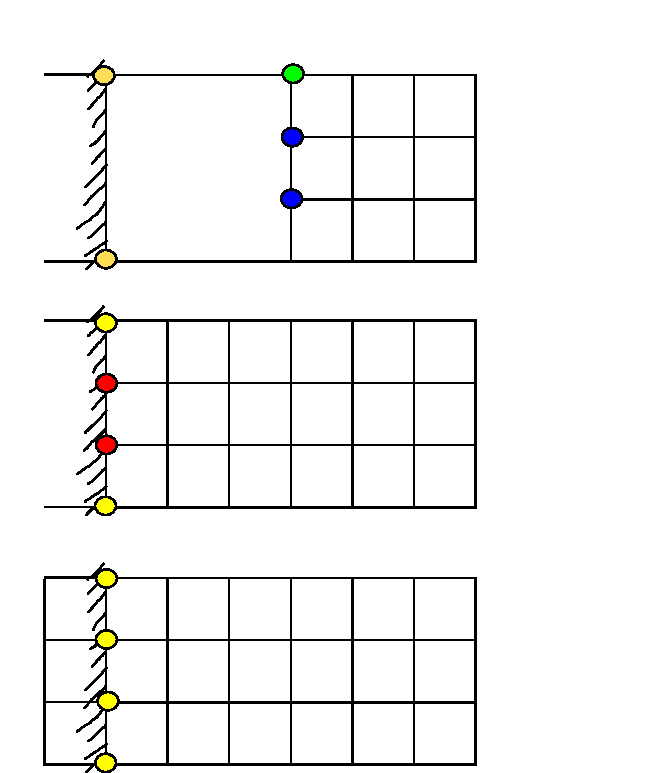
\includegraphics[width=0.5\textwidth]{98_patterns/boundaries-without-hanging-nodes.pdf}
\end{center}

\noindent
The algorithmic pattern is straightforward to implement with the vertex analysis
routines.
Please note that this code fragment/pattern also erases along the boundary:
\begin{code}
#include "peano/grid/aspects/VertexStateAnalysis.h"

void boxmg::mappings::RefinementCriterion::leaveCell( ...) {
 if (fineGridCell.isRefined()) {
  bool oneInnerVertexIsRefined      = false;
  bool allInnerVerticesAreUnrefined = true;
  dfor2(k)
   oneInnerVertexIsRefined |= 
    (
    fineGridVertices[ fineGridVerticesEnumerator(k) ].isInside() 
    &&
    fineGridVertices[ fineGridVerticesEnumerator(k)].getRefinementControl()
     ==Vertex::Records::Refined
    ); 
   allInnerVerticesAreUnrefined &= 
    (
    !fineGridVertices[ fineGridVerticesEnumerator(k) ].isInside()
    ||
    fineGridVertices[ fineGridVerticesEnumerator(k)].getRefinementControl()
     ==Vertex::Records::Unrefined
    ); 
  enddforx

  // ensure boundary is refined
  if (oneInnerVertexIsRefined) {
   dfor2(k)
    if (
     fineGridVertices[ fineGridVerticesEnumerator(k) ].isBoundary() &&
     fineGridVertices[ fineGridVerticesEnumerator(k) ].getRefinementControl() 
      == exahype::Vertex::Records::Unrefined) { 
      fineGridVertices[fineGridVerticesEnumerator(k) ].refine(); 
    }
   enddforx
  }
  
  // erase boundary again
  if (allInnerVerticesAreUnrefined) {
   dfor2(k)
    if (
     fineGridVertices[ fineGridVerticesEnumerator(k) ].isBoundary() &&
     fineGridVertices[ fineGridVerticesEnumerator(k) ].getRefinementControl() 
      == exahype::Vertex::Records::Refined) { 
      fineGridVertices[fineGridVerticesEnumerator(k) ].erase(); 
    }
   enddforx
  }
 }    
}
\end{code}
